\documentclass[unicode,11pt,a4paper,oneside,numbers=endperiod,openany]{scrartcl}

\usepackage{assignment}
\usepackage{textcomp}
\hyphenation{PageRank}
\hyphenation{PageRanks}

\usepackage{listings}
\usepackage{color} %red, green, blue, yellow, cyan, magenta, black, white
\definecolor{mygreen}{RGB}{28,172,0} % color values Red, Green, Blue
\definecolor{mylilas}{RGB}{170,55,241}


\begin{document}

\lstset{language=Matlab,%
    %basicstyle=\color{red},
    basicstyle=\ttfamily\tiny,
    breaklines=true,%
    morekeywords={matlab2tikz},
    keywordstyle=\color{blue},%
    morekeywords=[2]{1}, keywordstyle=[2]{\color{black}},
    identifierstyle=\color{black},%
    stringstyle=\color{mylilas},
    commentstyle=\color{mygreen},%
    showstringspaces=false,%without this there will be a symbol in the places where there is a space
    numbers=left,%
    numberstyle={\tiny \color{black}},% size of the numbers
    numbersep=9pt, % this defines how far the numbers are from the text
    emph=[1]{for,end,break},emphstyle=[1]\color{red}, %some words to emphasise
    %emph=[2]{word1,word2}, emphstyle=[2]{style},    
}

\setassignment
\setduedate{Monday 10 October 2016}
\serieheader{
Software Atelier: Differential Equations}{Academic Year 2016/2017}{Instructor: Dr. Drosos Kourounis}{TA: Hardik Kothari}{Assignment 3 - FEM implementation}{}
\newline


\begin{center}
\begin{tabular}{rc}
Name: Juraj Kardos   & \rule{5cm}{0.0pt} \\
Discussed with: & \rule{5cm}{0.0pt} 
\end{tabular}
\end{center}



\section{The Problem}
We seek the discrete solution of Poisson's equation
\begin{align}
    -\nabla^2 u(x,y) &= f(x,y),\ (x,y) \in \Omega \\
    u &= u_0,\ (x,y) \in \partial\Omega.
\end{align}

We want the exact solution of the PDE to be 
\begin{equation}
u_0(x,y) = 10x + tanh(10x-10)
\end{equation}

so we can compute $f(x,y)$ as following:
\begin{lstlisting}
syms x;
u = -(10*x + tanh(10*x - 10));
diff(u,x,2)

>> ans = -20*tanh(10*x - 10)*(10*tanh(10*x - 10)^2 - 10)
\end{lstlisting}

\section{FEM Solution}

\subsection{Mesh Generation}

The solution starts with generation of the mesh that approximates our domain. We assume unit square with non-overlapping elements. The domain is discretized by $N_x$ by $N_y$ grid of nodes. These nodes are then used as vertices of the elements. We either use quadrilateral or triangle elements, depending on the last parameter of the method \texttt{makeGrid(L\_x, L\_y, N\_x, N\_y, grid\_type)}. In case of triangular mesh each quadrilateral is simply split into two triangles by drawing the diagonal between local points 1 and 3.


\noindent\begin{minipage}{.45\textwidth}
\begin{lstlisting}[caption=Triangular mesh,frame=tlrb]{Name}
[...]
if(strcmp(grid_type, `triangles`))
    N_v = 3;
    N_e = (N_x-1)*(N_y-1)*2;
    elements(id_elem,:) = [e, e+1, e+N_x+1];
    elements(id_elem + 1,:) = [e, e+N_x+1, e+N_x];
    id_elem = id_elem + 2;
end
[...]
\end{lstlisting}
\end{minipage}\hfill
\begin{minipage}{.45\textwidth}
\begin{lstlisting}[caption=Quadrilateral mesh,frame=tlrb]{Name}
[...]
if(strcmp(grid_type, `quadrilaterals`))
    N_v = 4;
    N_e = (N_x-1)*(N_y-1);
    %follow convenction when enumerating the corners of the element
    elements(id_elem,:) = [e, e+1, e+N_x+1, e+N_x];
    id_elem = id_elem + 1;
end
[...]
\end{lstlisting}
\end{minipage}

\subsection{Assembly of Discrete Operators}
\begin{lstlisting}
%generate triangular grid
mesh = makeGrid(1,1,N,N,'triangles');
%or alternatively use quadrilaterals
mesh = makeGrid(1,1,N,N,'quadrilaterals');

%% assemble FEM operators 
[M, K, b] = assembleDiscreteOperators(mesh);
\end{lstlisting}

Next step in FEM is assembly of discrete operators, namely mass matrix $M$, laplacian matrix $K$ and discretized RHS $b$. The idea of the assembly is to construct the local versions of the matrices and insert them into the global structure. 

\subsubsection{Mass Matrix}
The assembly of mass matrix comes from projecting RHS function $f$ into the basis function space (see assembly of RHS below). We discretize integral over the whole domain and further broke it down into the sum of integrals over the individual elements.
\begin{equation}
    M_{ij} = \int_V N_i N_j dV = \sum_{e=1}^{N_e} \int_{V^e} N_i N_j dV^e
\end{equation}

% The local mass matrix comes from discretization of the identity matrix in the equation:
% \begin{equation}
%     u = f,
% \end{equation}
% which becomes
% \begin{equation}
%     Mu_d = f_d,
% \end{equation}
% where $u_d$ is discretized solution defined only in the nodes of the grid and interpolated by combination of nodal values and basis functions elsewhere:
% \begin{equation}
%     u_d = \sum_{j}^{} u_j N_j.
% \end{equation}
% After applying the projection to the basis function space and forming the weak formulation, the LHS of the above problem becomes the mass matrix $M$ multiplied by the discretized solution $u_d$.

To simplify the assembly of the local matrix, instead of the quadrature we can use shorthand equation to determine the integrand explicitly using the formula (applies for 2D triangular mesh):
\begin{equation}
    m_{ij} = \int_{V^e} N_i N_j  dV^e = \frac{d!V_i^e!I!J!}{(d+I+J)!}
\end{equation}
where
\begin{align}
    I,J &= 1 \text{ \ \  \ \ \ if } i\neq j \\
    I &= 2 \text{ \ \  \ \ \ if } i = j \\
    J &= 0 \\
    V^e &= \frac{1}{d!} abs (det (
    \begin{matrix}
    x_1 & y_1 & 1 \\
    x_2 & y_2 & 1 \\
    x_3 & y_3 & 1 \\
    \end{matrix}))
\end{align}

\noindent\begin{minipage}{.45\textwidth}
\begin{lstlisting}[caption=Triangular $m_e$,frame=tlrb]{Name}
%use formula for mass matrix
Me = ...
    [1/6 1/12 1/12;
     1/12 1/6 1/12;
     1/12 1/12 1/6];
 
 %get volume of the element
 nodes = mesh.Elements(e,:);
 coords = ones(3,3);
 coords(:,1) = mesh.Points(nodes,1); %x coords
 coords(:,2) = mesh.Points(nodes,2); %y coords
 Ve = 1/2 * abs(det(coords));
 
 Me = Me * Ve;
\end{lstlisting}
\end{minipage}\hfill
\begin{minipage}{.45\textwidth}
\begin{lstlisting}[caption=Quadrilateral $m_e$,frame=tlrb]{Name}
%result from the Msymbolic.m for quadrilateral mesh

Me = ... 
[  (dx*dy)/9, (dx*dy)/18, (dx*dy)/36, (dx*dy)/18;
   (dx*dy)/18,  (dx*dy)/9, (dx*dy)/18, (dx*dy)/36;
   (dx*dy)/36, (dx*dy)/18,  (dx*dy)/9, (dx*dy)/18;
   (dx*dy)/18, (dx*dy)/36, (dx*dy)/18,  (dx*dy)/9  ];
\end{lstlisting}
\end{minipage}

\subsubsection{Stiffness matrix}
After forming the weak formulation and projecting the laplace operator into the space of test function and discretization we form the equation where the gradients of the basis function show up:
\begin{equation}
    LHS = \sum_{i=0}^{N_e} u_i \int_{V^e} \nabla N_i \nabla N_j dV^e
\end{equation}

We use linear basis functions $N_i(x,y) = a_ix + b_iy + c_i$ with the gradient $\nabla N_i = [a_i, b_i]$. The integral over the element becomes
\begin{equation}
    k_{ij} = \int_{V^e} \nabla N_i \nabla N_j dV^e = V^e (a_ia_j + b_ib_j).
\end{equation}
The entries of the local laplacian matrix may then be computed by using outer product of coefficients of basis functions as shown in the code below that forms local $k_e$ for triangular mesh.

\noindent\begin{minipage}{.38\textwidth}
\begin{lstlisting}[caption=Triangular $k_e$,frame=tlrb]{Name}
%find coeff. matrix, which is the inverse of barycentric coordinates
nodes = mesh.Elements(e,:); 
coords = ones(3,3);
coords(:,1) = mesh.Points(nodes,1); %x coords
coords(:,2) = mesh.Points(nodes,2); %y coords
coeff = inv(coords);

%make grad Ni; grad(Ni) * grad(Nj)
%make integral -> (ai*aj + bi*bj)*V
ai = coeff(1,:);
bi = coeff(2,:);

%use outer product
Ke = ai'*ai + bi'*bi;

%get volume of the element
Ve = 1/2 * abs(det(coords));
Ke = Ke * Ve;
\end{lstlisting}
\end{minipage}\hfill
\begin{minipage}{.51\textwidth}
\begin{lstlisting}[caption=Quadrilateral $k_e$,frame=tlrb]{Name}
%result from the Msymbolic.m for quadrilateral mesh

Ke = ... 
[  (dx^2 + dy^2)/(3*dx*dy),    dx/(6*dy) - dy/(3*dx), -(dx^2 + dy^2)/(6*dx*dy),    dy/(6*dx) - dx/(3*dy);
    dx/(6*dy) - dy/(3*dx),  (dx^2 + dy^2)/(3*dx*dy),    dy/(6*dx) - dx/(3*dy), -(dx^2 + dy^2)/(6*dx*dy);
 -(dx^2 + dy^2)/(6*dx*dy),    dy/(6*dx) - dx/(3*dy),  (dx^2 + dy^2)/(3*dx*dy),    dx/(6*dy) - dy/(3*dx);
    dy/(6*dx) - dx/(3*dy), -(dx^2 + dy^2)/(6*dx*dy),    dx/(6*dy) - dy/(3*dx),  (dx^2 + dy^2)/(3*dx*dy)];
\end{lstlisting}
\end{minipage}

After forming the local mass and laplacian matrix for each element, we need to insert these into the global matrices $M$ and $K$. The insertion is done based on local-global correspondence between node numbering. 
\begin{lstlisting}
%assembly of local matrices into global structure
N = mesh.N;
N_e = mesh.N_e;
N_v = mesh.N_v;

M = zeros(N,N) ;
K = zeros(N,N) ;

for e = 1:N_e
    % M_e element mass matrix
    % K_e element Laplacian
    Me = makeMe(e, mesh);
    Ke = makeKe(e, mesh);
    for i = 1:N_v
        I = mesh.Elements(e, i);
        for j = 1:N_v
            J = mesh.Elements(e, j);
            M(I, J) = M(I, J) + Me(i, j);
            K(I, J) = K(I, J) + Ke(i, j);
        end
    end
end
\end{lstlisting}

\subsubsection{RHS}
FEM computes the value of the target function only in the nodes and the values inside the elements are linearly interpolated. The values of the target function inside the element are:
\begin{equation}
    f^e(x,y) = f^e(x_1,y_1) * N_1(x,y) + f^e(x_2,y_2) * N_2(x,y) + f^e(x_3,y_3) * N_3(x,y) 
\end{equation}

Projecting and discretizing the RHS of the original problem, we get following formulation. We use local mass matrix $m_{ij} = \int_{V^e} N_i N_j $:
\begin{equation}
    \int_V f N_j dV = \sum_{e=1}^{N_e} \int_{V^e} f^e N_j dV^e = \sum_{e=1}^{N_e} \int_{V^e} \sum_i (f_i N_i) N_j dV^e = \sum_{e=1}^{N_e} \sum_i f_i m_{ij}
\end{equation}

\begin{lstlisting}[caption=Assembly of RHS]
for e = 1:N_e
    I = mesh.Elements(e,:);
    Xe = mesh.Points(I,1);
    Ye = mesh.Points(I,2);

    be = f(Xe,Ye);
    be = Me*fp;

    for i = 1:N_v
        I = mesh.Elements(e, i);
        b(I) = b(I) + be(i);
    end
end
\end{lstlisting}

\subsection{Boundary Conditions}
We need to modify the equations for the points that lie on the boundary of our domain. The Dirichlet boundary specifies exact value of the target profile, that is $u(x,y) = u_0(x,y)$ for every $(x,y) \in \partial\Omega$. What that means in practice is that we need to know which points belong to the boundary and change laplacian matrix $K$ accordingly.
\begin{lstlisting}
% impose boundary conditions for Dirichlet boundaries
markers = reshape(mesh.PointMarkers,[mesh.N,1]);
boundaryPoints = find(markers);

% 1 on diagonal, 0 elsewhere
K(boundaryPoints,:) = 0;
K(boundaryPoints,boundaryPoints) = diag(ones(size(boundaryPoints,1),1)); %diagonal

% u0 as RHS
X = mesh.Points(boundaryPoints,1);
Y = mesh.Points(boundaryPoints,2);
b(boundaryPoints) = u0(X,Y);
\end{lstlisting}

\subsection{Solution}
Having the system ready at hand, we need to solve it. In vector $u$ we will have approximate solution to our problem.
\begin{lstlisting}
% solve
u = K\b;

% visualize solution
writeMeshToVTKFile(mesh, x, 'solution')
\end{lstlisting}


\subsection{Visualization of the Solution}
\begin{figure}[h]
    \centering
    \includegraphics[width=0.85\textwidth]{../triangles}
    \caption{Triangular mesh $100 \times 100$ and FEM solution.}
    \label{fig:mesh_tr}
\end{figure}

\begin{figure}[h]
    \centering
    \includegraphics[width=0.95\textwidth]{../quadrilaterals}
    \caption{Quadrilateral mesh $100 \times 100$ and FEM solution.}
    \label{fig:mesh_quad}
\end{figure}

\begin{figure}[h]
    \centering
    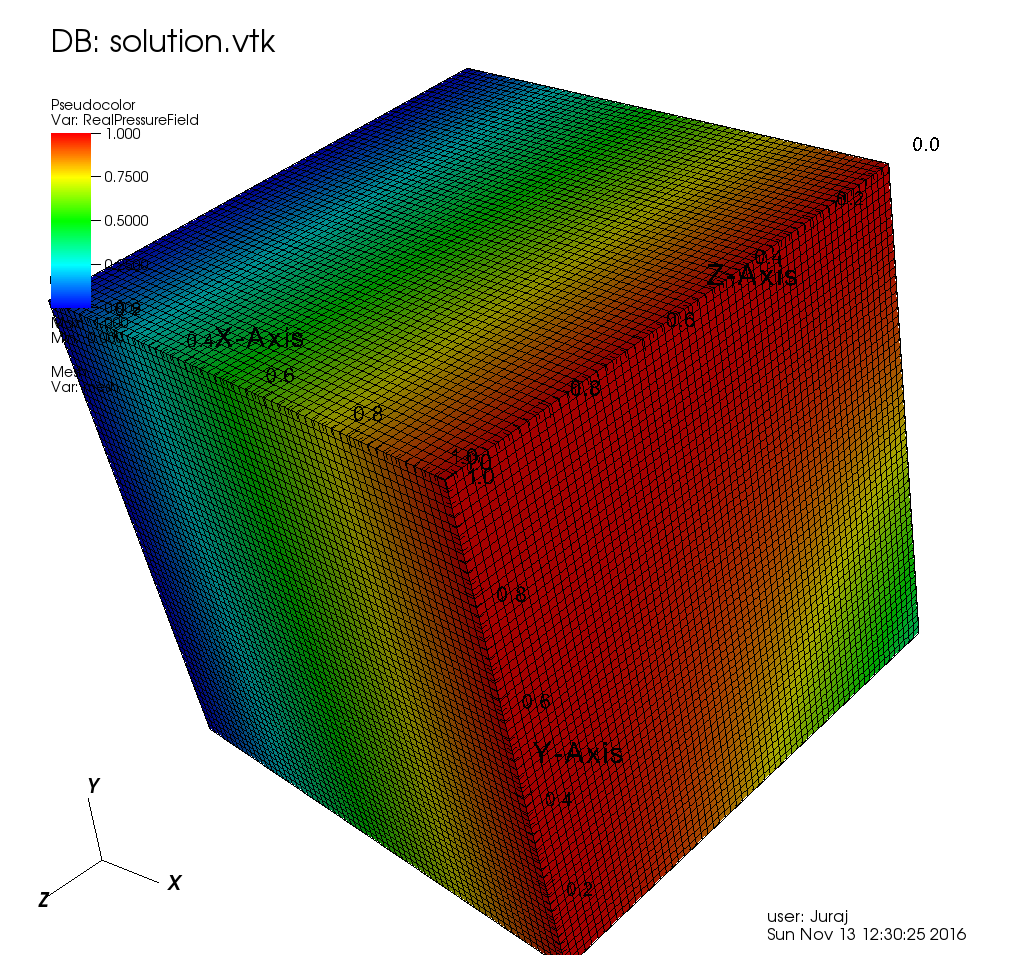
\includegraphics[width=0.95\textwidth]{../solution}
    \caption{Exact solution.}
    \label{fig:solution}
\end{figure}

\begin{figure}[h]
    \centering
    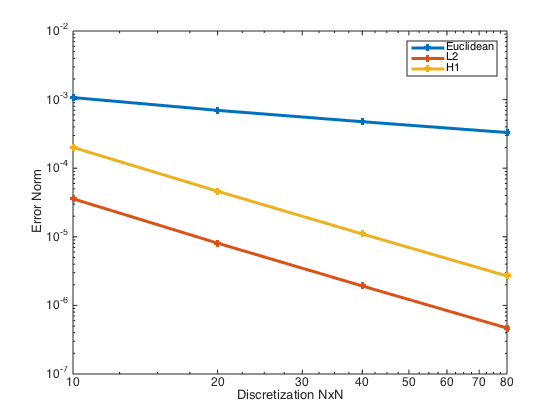
\includegraphics[width=0.95\textwidth]{../FEMerror}
    \caption{Error norms for discretizations \texttt{50:25:150}}
    \label{fig:norms}
\end{figure}

\end{document}
